\documentclass[12pt, french]{article}
\usepackage{graphicx}
\usepackage[T1]{fontenc}
\usepackage[utf8]{inputenc}
\usepackage{lmodern}
\usepackage{amsfonts}
\usepackage{enumitem}
\usepackage[a4paper]{geometry}
\usepackage{babel}
\usepackage{wrapfig}
\usepackage[figurename=Fig.]{caption}
\usepackage{subfig}

\usepackage{color}   %May be necessary if you want to color links
\usepackage{hyperref}
\hypersetup{
    colorlinks=true, %set true if you want colored links
    linktoc=all,     %set to all if you want both sections and subsections linked
    linkcolor=blue,  %choose some color if you want links to stand out
}

\begin{document}
\renewcommand{\labelitemi}{$\bullet$}
	\begin{titlepage}
		
		\newcommand{\HRule}{\rule{\linewidth}{0.4mm}} % Defines a new command for the horizontal lines, change thickness here
		
		\center % Center everything on the page
		
		%----------------------------------------------------------------------------------------
		%	HEADING SECTIONS
		%----------------------------------------------------------------------------------------
		
		\textsc{\LARGE Université de Montréal}\\[1cm] % Name of your university/college
		\textsc{\Large Faculté des arts et des sciences}\\[0.5cm] % Major heading such as course name
		\textsc{\large Département d’informatique et de recherche opérationnelle (DIRO) }\\[0.3cm] % Minor heading such as course title
		
		%----------------------------------------------------------------------------------------
		%	TITLE SECTION
		%----------------------------------------------------------------------------------------
		
		\HRule \\[0.4cm]
		{ \huge Rapport de stage \\ \bfseries Évaluation du risque de retour à la maison } \\[0.4cm] % Title of your document
		\HRule \\[1.5cm]
		
		%----------------------------------------------------------------------------------------
		%	AUTHOR SECTION
		%----------------------------------------------------------------------------------------
		
		\begin{minipage}{0.4\textwidth}
			\begin{flushleft} \large
				\emph{Auteur:}\\
				Vilon \textsc{Saint-Fleurose} % Your name
				\\MSc, informatique \\Université de Montréal
			\end{flushleft}
		\end{minipage}
		~
		\begin{minipage}{0.4\textwidth}
			\begin{flushright} \large
				\emph{Directeur de recherche:} \\
				Dr. Michalis \textsc{Famelis} % Supervisor's Name
				\\Professeur adjoint \\Université de Montréal
			\end{flushright}
		\end{minipage}\\[1cm]
			~
			\begin{minipage}{0.4\textwidth}
				\begin{center} \large
					\emph{Superviseur:} \\
					 Nicolas \textsc{Coallier} % Supervisor's Name
					\\Vice-Président Exécutif, TIC \\ML+
				\end{center}
			\end{minipage}\\[1cm]
		
		% If you don't want a supervisor, uncomment the two lines below and remove the section above
		%\Large \emph{Author:}\\
		%John \textsc{Smith}\\[3cm] % Your name
		
		%----------------------------------------------------------------------------------------
		%	DATE SECTION
		%----------------------------------------------------------------------------------------
		
		{\large \today}\\[1cm] % Date, change the \today to a set date if you want to be precise
		
		%----------------------------------------------------------------------------------------
		%	LOGO SECTION
		%----------------------------------------------------------------------------------------
		
		
\includegraphics[width=3cm, height=1cm]{logo.png} % Include a department/university logo - this will require the graphicx package
		
		%----------------------------------------------------------------------------------------
		
		\vfill % Fill the rest of the page with whitespace
		
	\end{titlepage}
		
\tableofcontents
\newpage	
\addcontentsline{toc}{section}{Remerciements}
\section*{Remerciements}
Je veux commencer d'abord par remercier le Grand Dieu Tout-Puissant, le Créateur de l'univers, des cieux et de la terre qui m'a donné la vie, la santé, les opportunités et tout ce dont j'avais besoin pour faire cette grande et belle étude à l'université de Montréal. Il a rendu toutes choses possibles en ma faveur, moi qui suis pécheur et désobéissant; immérité de toutes ces grâces. Il m'accompagnait toujours dans les moments les plus difficiles de ma vie, Il ne m'a jamais laissé seul; surtout dans les moments où je devais payer les frais de scolarité qui étaient si énormes et impossibles à payer de mon propre compte. A un Dieu si merveilleux et si bon, je Lui dois beaucoup de reconnaissance.  \\
	
	Je remercie aussi ma femme qui m'a beaucoup supporté pendant plus de deux années d'études. Elle n'a jamais murmuré, ni découragé quand nous devions passer par des moments difficiles de notre vie conjugale à cause de ces études. Elle a mis toutes ses ressources disponibles pour entretenir la famille et payer mes études quand j’étais moi-même dans l’impossibilité de travailler. Vraiment, ma femme est une bénédiction dans ma vie, un cadeau venant de Dieu. Je t’aime ma chérie. \\
	
	Je tiens à remercier le professeur Michalis Famelis d’avoir accepté être mon directeur de recherche et supervisé ce stage, il est toujours là pour m’encourager et me pousser vers l’avant. Il répond toujours présent à tous mes appels, il est toujours disponible pour me rencontrer, me parler et me conseiller ; même en dehors du cadre universitaire.  \\
	
	Je remercie Nicolas Coallier et toute l’équipe ML+ qui ont accepté que je sois leur stagiaire, ils ont placé  leur confiance en moi quoiqu’ils ne me connaissaient pas encore. Cette équipe, quoique jeune, est très dynamique et chaleureuse, c’est une équipe motivante qui stimule la connaissance. J’ai dû apprendre beaucoup de choses par rapport à eux.
	Finalement, je présente mes sincères remerciements à toute la communauté universitaire, à DIRO en particulier. Merci pour la formation prestigieuse que vous m’avez fournie. Cette formation est si solide qu’elle m’aidera rapidement à intégrer le marché du travail sans perdre de temps. 
	
\newpage

\listoffigures


\newpage

\addcontentsline{toc}{section}{Résumé}
\section*{Résumé}
L'arthroplastie totale de la hanche et du genou réduit considérablement la douleur
et améliore la fonction chez les personnes atteintes d'arthrose avancée. le
vieillissement de la génération du "baby boom", combiné au désir de
maintenir un mode de vie actif et sans douleur, entraînera une augmentation
du nombre annuel de chirurgies de remplacement articulaire pratiquées dans
États Unis. L'Académie américaine des chirurgiens orthopédiques a
projeté que d'ici 2030, les arthroplasties totales de la hanche et du genou
augmentera à plus de 748 000 / an. 
Avec l'augmentation continue du nombre de chirurgies de remplacement, il devient crucial aux administrateurs des hôpitaux de déterminer si les patients doivent rester à l'hôpital pour une réadaptation après leur 	chirurgie ou s'ils doivent être renvoyés à la maison puisque les coûts associés à une réadaptation doivent être pris en charge par les hôpitaux. Il est important de souligner que la majorité des compagnies d'assurance santé aux États Unis n'assument pas les coûts liés à la réadaptation des patients. Ces frais qui sont très élevés (entre 15-30,000 \$ par patient) doivent être assurés par les hôpitaux. Pour prendre la décision de retour ou non, les chirurgiens tiennent compte des antécédents médicaux du patient, ce qui est un travail difficile à effectuer manuellement. Dans notre projet de stage, nous développerons un model de machine learning qui aide à prendre cette décision de façon automatique.
   	
\newpage
\section{Introduction}	
	
Le système de santé aux USA repose sur deux types de financement. Premièrement, sur le financement public qui englobe certains groupes de personnes de la population américaine uniquement. Il se concentre 	essentiellement sur deux programmes : le programme 		fédéral Medicare pour les plus de 65 ans et les personnes gravement handicapées (soit 15 \% de la population) et le programme Medicaid qui 			s’adresse aux familles pauvres avec enfants et touche 11 \% de la population. Deuxièmement, sur le financement privé qui touche tout le reste de la population, l’assurance est donc majoritairement privée aux 		Etats-Unis. Les Américains sont assurés en général via leurs employeurs ou sinon de manière individuelle lorsque leur employeur ne propose pas d’assurance ou qu’ils travaillent en indépendant. La composante « 	assurance médicale » dans le choix d’un emploi est donc un critère important.\\
	
Le système américain, libéral et fondé sur le marché, s’organise autour d’assurances privées souvent liées à l’emploi et d’une assurance maladie obligatoire, liée notamment à la vieillesse et aux faibles revenus.
Cependant, ce système, qui n’est pas universel, échoue à couvrir l’intégralité de la population, dont une partie se retrouve sans assurance santé.\\

Les compagnies d'assurance privées ne couvrent pas les coûts associés à une réadaptation d'un patient après une arthroplastie (Opération ayant pour but de rétablir la forme et la mobilité d'une articulation abîmée ou bloquée.). Il revient à l'hôpital de couvrir ces coûts qui sont très élevés d'après le docteur orthopédiste Jonah Hebert-Davies qui a fait ses études de spécialité en Orthopédie à l'université de Seattle, Washington USA. Selon le docteur les coûts estimés sont entre 15 à 30,000 \$ par patient. Ce qui revient à une grande perte financière pour les hôpitaux.  La décision de maintenir ou de renvoyer un patient après une arthroplastie devient une question préoccupante dans la mesure où elle pourrait réduire le coût budgétaire des hôpitaux. Si la décision prise est de renvoyer le patient, l'hôpital est le gagnant sinon il est le perdant\\ 

D'autres part, l'arthrose (maladie qui touche les articulations et caractérisée par la douleur et la difficulté à effectuer des mouvements articulaires) touche environ 27 millions d'adultes aux États-Unis.  Ce qui augmente considérablement le nombre d'arthroplastie dans les hôpitaux, et aussi le poids de travail des médecins à savoir quand est-ce qu'il ya une réadaptation ou non.\\

Il est un travail fastidieux pour les spécialistes orthopédistes de vérifier manuellement les données médicales d'un patient pour pouvoir décider s'il doit être renvoyé ou non. Ce travail consiste en ce que les données médicales d'un dossier patient sont très volumineuses. Créer un moyen d'automatiser ce processus est le but de notre projet.  \\

Nous supposons qu'il existe déjà un jeu de données disponibles contenant toutes les informations touchant un grand nombre de patients et que chaque échantillon de ce jeu de données est un dossier patient. Nous supposons aussi que ce jeu de données possède des caractéristiques suffisantes pour décider si un patient doit être renvoyé ou non. Nous considérons aussi que ce jeu de données est composé de patients qui font l'objet d'une décision de retour. Si toutes ces conditions sont réunies, nous pouvons profiter des différentes technologies de la science de données en général et du marching learning en particulier pour développer un outil d'aide à la décision qui aide les orthopédistes à prendre la décision de retour automatiquement. \\

La suite de ce rapport est composé de plusieurs sections et chaque section peut avoir des subsections. La section 2 donne un contexte théorique des différents éléments qui sont importants pour notre projet. La section 3 présente en détail une description technique des différentes étapes de notre projet. La section 4 fait une évaluation de notre outil crée. La section 5 présente les limitations et les travaux futurs. La section 6 détaille les travaux connexes et la section 7 est celle de la conclusion.


\newpage

\section{Contexte théorique}

Dans cette section nous voulons présenter une approche théorique des différents concepts que nous avons utilisés dans le cadre notre projet. Nous allons faire un résumé de chaque concept important que nous avons utilisé dans le cadre de l'implémentation de ce projet. Nous n'allons pas toucher tout ce qui a rapport aux concepts mais juste ce qui nous intéresse et util pour le projet. Il y aura des références pour ceux qui veulent approfondir les concepts. 

\subsection{Sciences des données}

La science des données est un domaine interdisciplinaire de méthodes, processus, algorithmes et systèmes scientifiques permettant d'extraire des connaissances ou des informations à partir de données sous diverses formes, structurées ou non. Elle emploie des techniques et des théories tirées de plusieurs autres domaines plus larges des mathématiques, la statistique principalement, la théorie de l'information et la technologie de l'information, notamment le traitement de signal, des modèles probabilistes, l'apprentissage automatique, l'apprentissage statistique, la programmation informatique, l'ingénierie de données, la reconnaissance de formes et l'apprentissage, la visualisation, l'analytique prophétique, la modélisation d'incertitude, le stockage de données, la compression de données et le calcul à haute performance. Les méthodes qui s'adaptent aux données de masse sont particulièrement intéressantes dans la science des données, bien que la discipline ne soit généralement pas considérée comme limitée à ces données.\\
	
L'objectif du « data scientist » (expert en données massives) est de produire des méthodes (automatisées, autant que possible) de tri et d'analyse de données de masse et de sources plus ou moins complexes ou disjointes de données, afin d'en extraire des informations utiles ou potentiellement utiles. 
Le métier de data scientist est apparu pour trois raisons principales :	
\begin{itemize}
\item l'explosion de la quantité de données produites et collectées par les humains;
\item 	l'amélioration et l'accessibilité plus grande des algorithmes de machine learning;
\item l'augmentation exponentielle des capacités de calcul des ordinateurs.\\
\end{itemize}	
Le cycle de travail du data scientist comprend notamment:
\begin{itemize}
\item la récupération des données utiles à l'étude;
\item le nettoyage des données pour les rendre exploitables;
\item une longue phase d'exploration des données afin de comprendre en profondeur l'articulation des données;
\item la modélisation des données;
\item l'évaluation et interprétation des résultats;
\item  la conclusion de l'étude : prise de décision ou déploiement en production du modèle.
\end{itemize}
L'image ci-dessous donne une vue générale du travail d'un data scientist. Étant stagiaire en science de données, nous avons suivi minutieusement, dans le cadre de notre projet, le cycle de travail complet du data scientist. Depuis la récupération des données jusqu'au déploiement d'un système en production. Nous expliquerons en détail dans la section "Aperçu", comment nous implémentons ce cycle au sein de notre projet. \\ \\
\begin{figure}[h]
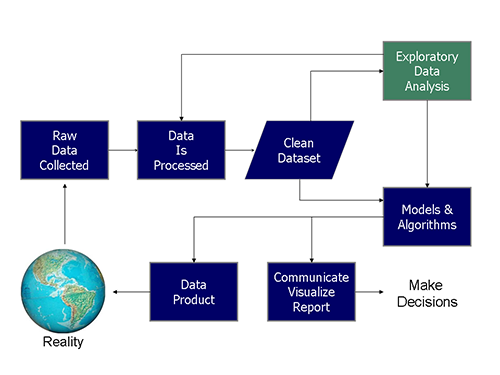
\includegraphics[]{workflow_datascientis.png}
\caption{work cycle of data scientist}
\end{figure}
Deux composantes sont nécessaires pour pouvoir commencer à se demander si la data science peut, oui ou non, apporter de la valeur et aider à la résolution d'un problème : des \textbf{données} et une \textbf{problématique} bien définie.
\paragraph{Données.}
 Les données constituent la ressource principale pour qu'un data scientist puisse effectuer son travail correctement. Nos données proviennent du département orthopédique de l'université de Seattle, Washington, États-Unis. Elles sont au nombre de 2718 files et 92 colonnes. Nous les utilisons comme données historiques (\textit{historical data, en anglais}) dans le cadre du développement de notre modèle de machine learning. 
\paragraph{Problématique.}
La problématique de notre projet, comme nous l'avons vu dans l'introduction, est d'aider à décider si un patient doit rester à l'hôpital ou rentrer chez lui après une arthroplastie.  

Au sein de ce cycle, le machine learning désigne l'ensemble des méthodes de modélisation statistique à partir des données, et se situe bien au coeur du travail du data scientist. Dans la sous-section qui suit nous allons aborder le machine learning, car le gros de notre travail est de construire un model machine learning d'aide à la décision. Nous verrons une brève introduction sur ce quoi le machine learning, ensuite un survol sur les concepts fondamentaux du ML et finalement nous nous concentrerons sur un sous-ensemble de concepts qui touchent notre projet, principalement le problème de classification. Nous n'aborderons pas dans ce rapport, la théorie sur l'exploration des données \textit{(data mining en anglais)}. Nous supposons que ceux qui lisent ce rapport ont déjà des notions élémentaires sur cette question, sinon ils peuvent visiter wikipedia ou n'importe quelle autre page pour avoir des idées générales sur ce point.

\subsection{Vue d'ensemble sur Machine Learning}

Dans la section précédente, nous avons pu y voir plus clair sur le cycle global de travail du data scientist. Nous allons maintenant parler du machine learning dans cette section, c'est à dire la modélisation des données. Nous utilisons le machine learning probablement des dizaines de fois par jour sans même le savoir. Chaque fois que nous effectuons une recherche Web sur Google ou Bing, cela fonctionne si bien c'est parce que leur logiciel de machine learning a trouvé comment classer les pages. Lorsque Facebook ou l'application photo d'Apple reconnaît nos amis dans nos images, c'est aussi du machine learning. Chaque fois que nous lisons notre courrier électronique et qu'un filtre anti-spam nous évite d'avoir à parcourir des tonnes de spam, c'est parce que nos ordinateurs ont appris à distinguer le spam du courrier non-spam. Donc, c'est du machine learning. C'est la science qui consiste à apprendre les ordinateurs sans être explicitement programmés. \\
Le machine learning constitue une manière de modéliser des phénomènes, dans le but de prendre des décisions stratégiques. Les algorithmes utilisés permettent, dans une certaine mesure, à un système piloté par ordinateur (un robot éventuellement), ou assisté par ordinateur, d'adapter ses analyses et ses comportements en réponse, en se fondant sur l'analyse de données empiriques provenant d'une base de données ou de capteurs. La difficulté réside dans le fait que l'ensemble de tous les comportements possibles compte tenu de toutes les entrées possibles devient rapidement trop complexe à décrire \textbf{(on parle d'explosion combinatoire)}. On confie donc à des programmes le soin d'ajuster un modèle pour simplifier cette complexité et de l'utiliser de manière opérationnelle. Idéalement, l'apprentissage visera à être non supervisé, c'est-à-dire que la nature des données d'entrainement n'est pas connue.
\begin{figure}[h]
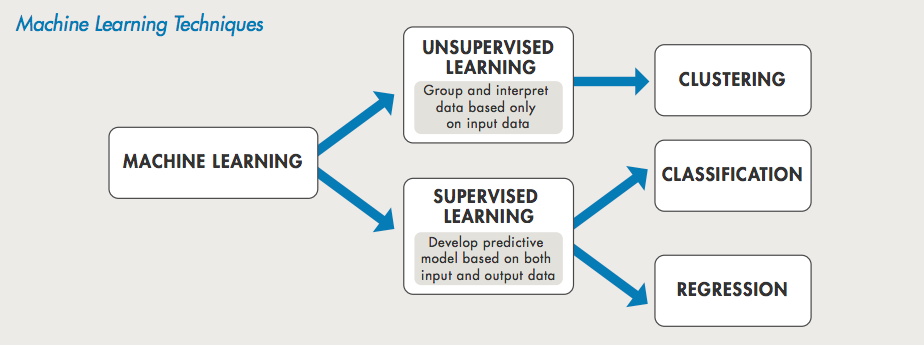
\includegraphics[width=15cm, height=6cm]{machinelearning.png}
\caption{Machine learning representation}
\end{figure}

Les algorithmes d'apprentissage peuvent se catégoriser selon le mode d'apprentissage qu'ils emploient :

\paragraph{Apprentissage supervisé. }

L'apprentissage supervisé (supervised learning en anglais) est une technique d'apprentissage automatique où l'on cherche à produire automatiquement des règles à partir d'une base de données d'apprentissage contenant des « exemples » (en général des cas déjà traités et validés).\\
Une base de données d'apprentissage (ou ensemble d'apprentissage) est un ensemble de couples entrée-sortie $(x_n, y_n)_{1 \leq n \leq N}$ avec $x_n \in X$ et $y_n \in Y $  , que l'on considère être tirées selon une loi sur $ X \times Y $ fixe et inconnue, par exemple $x_n$ suit une loi uniforme et $ y_n = f(x_n) + w_n$ où $w_n$ est un bruit centré. \\\\
On distingue trois types de problèmes solubles avec une méthode d'apprentissage automatique supervisée :  

\begin{itemize} 
\item $Y \subset \mathbb{R}$  : lorsque la sortie que l'on cherche à estimer est une valeur dans un ensemble continu de réels, on parle d'un problème de régression. La fonction de prédiction est alors appelée un régresseur.
\item $Y = \{ 1, \cdots, I \} $ lorsque l'ensemble des valeurs de sortie est fini, on parle d'un problème de classification, qui revient à attribuer une étiquette à chaque entrée. La fonction de prédiction est alors appelée un classifieur (ou classificateur).
\item Lorsque  $Y$ est un ensemble de données structurées, on parle d'un problème de prédiction structurée, qui revient à attribuer une sortie complexe à chaque entrée. Par exemple, en bio-informatique le problème de prédiction de réseaux d’interactions entre gènes peut être considéré comme un problème de prédiction structurée dans laquelle l'ensemble possible des sorties structurées est l'ensemble de tous les graphes modélisant les interactions possibles.
\end{itemize}




%si les classes sont prédéterminées et les exemples connus, le système apprend à classer selon un modèle de classement ; on parle alors d'apprentissage supervisé (ou d'analyse discriminante). Un expert (ou oracle) doit préalablement étiqueter des exemples. Le processus se passe en deux phases. Lors de la première phase (hors ligne, dite d'apprentissage), il s'agit de déterminer un modèle des données étiquetées. La seconde phase (en ligne, dite de test) consiste à prédire l'étiquette d'une nouvelle donnée, connaissant le modèle préalablement appris. Parfois il est préférable d'associer une donnée non pas à une classe unique, mais une probabilité d'appartenance à chacune des classes prédéterminées (on parle alors d'apprentissage supervisé probabiliste).\\
%ex. : L'analyse discriminante linéaire ou les SVM en sont des exemples typiques. Autre exemple : en fonction de points communs détectés avec les symptômes d'autres patients connus (les exemples), le système peut catégoriser de nouveaux patients au vu de leurs analyses médicales en risque estimé (probabilité) de développer telle ou telle maladie.

\paragraph{Apprentissage non supervisé.}
 
Quand le système ou l'opérateur ne disposent que d'exemples, mais non d'étiquettes, et que le nombre de classes et leur nature n'ont pas été prédéterminés, on parle d'apprentissage non supervisé ou clustering. Aucun expert n'est requis. L'algorithme doit découvrir par lui-même la structure plus ou moins cachée des données. Le partitionnement de données, data clustering en anglais, est un algorithme d'apprentissage non supervisé.\\
Le système doit ici — dans l'espace de description (la somme des données) — cibler les données selon leurs attributs disponibles, pour les classer en groupe homogènes d'exemples. La similarité est généralement calculée selon une fonction de distance entre paires d'exemples. C'est ensuite à l'opérateur d'associer ou déduire du sens pour chaque groupe et pour les motifs (patterns en anglais) d'apparition de groupes, ou de groupes de groupes, dans leur « espace ». Divers outils mathématiques et logiciels peuvent l'aider. On parle aussi d'analyse des données en régression (ajustement d'un modèle par une procédure de type moindres carrés ou autre optimisation d'une fonction de coût). Si l'approche est probabiliste (c'est-à-dire que chaque exemple, au lieu d'être classé dans une seule classe, est caractérisé par un jeu de probabilités d'appartenance à chacune des classes), on parle alors de « soft clustering » (par opposition au « hard clustering »).\\
Cette méthode est souvent source de sérendipité(le fait de réaliser une découverte scientifique ou une invention technique de façon inattendue à la suite d'un concours de circonstances fortuit )\\
ex. : Pour un épidémiologiste qui voudrait dans un ensemble assez large de victimes de cancer du foie tenter de faire émerger des hypothèses explicatives, l'ordinateur pourrait différencier différents groupes, que l'épidémiologiste chercherait ensuite à associer à divers facteurs explicatifs, origines géographique, génétique, habitudes ou pratiques de consommation, expositions à divers agents potentiellement ou effectivement toxiques (métaux lourds, toxines telle que l'aflatoxine, etc.).

\paragraph{Apprentissage semi-supervisé. }
Effectué de manière probabiliste ou non, il vise à faire apparaître la distribution sous-jacente des exemples dans leur espace de description. Il est mis en œuvre quand des données (ou « étiquettes ») manquent… Le modèle doit utiliser des exemples non étiquetés pouvant néanmoins renseigner.
Ex. : En médecine, il peut constituer une aide au diagnostic ou au choix des moyens les moins onéreux de tests de diagnostic.
Apprentissage partiellement supervisé 
probabiliste ou non, quand l'étiquetage des données est partiel3. C'est le cas quand un modèle énonce qu'une donnée n'appartient pas à une classe A, mais peut-être à une classe B ou C (A, B et C étant 3 maladies par exemple évoquées dans le cadre d'un diagnostic différentiel).
\paragraph{Apprentissage par renforcement.}l'algorithme apprend un comportement étant donné une observation. L'action de l'algorithme sur l'environnement produit une valeur de retour qui guide l'algorithme d'apprentissage.
ex. : L'algorithme de Q-learning est un exemple classique.
\paragraph{Apprentissage par transfert.}
L’apprentissage par transfert peut être vu comme la capacité d’un système à reconnaître et appliquer des connaissances et des compétences, apprises à partir de tâches antérieures, sur de nouvelles tâches ou domaines partageant des similitudes. La question qui se pose est : comment identifier les similitudes entre la ou les tâche(s) cible(s) et la ou les tâche(s) source(s), puis comment transférer la connaissance de la ou des tâche(s) source(s) vers la ou les tâche(s) cible(s) ?
\paragraph{Notion de dataset.}
Le dataset est l'ensemble des données utilisé pour entraîner un modèle. Il existe deux types de jeux de données (dataset) généraux. Jeux étiqueté et jeux sans étiquette.
\paragraph{Training Set and Test Set.}
Dans l'apprentissage automatique, un jeu de données universel inconnu est supposé exister, qui contient toutes les paires de données possibles ainsi que leur distribution de probabilité d'apparition dans le monde réel. Alors que dans les applications réelles, ce que nous avons observé est seulement un sous-ensemble de l'ensemble de données universel en raison du manque de mémoire ou d'un autre inévitable les raisons. Cet ensemble de données acquises s'appelle l'ensemble d'apprentissage \textbf{(Training Set)} et est utilisé pour apprendre les propriétés et la connaissance de l'ensemble de données universel. Afin d'examiner la performance de l'apprentissage, un autre ensemble de données peut être réservé pour le test, appelé ensemble de test ou données de test \textbf{(Test Set)}.\\
%\begin{itemize}
%\item Dataset étiqueté: $\mathbb{D}: X = \{x^{(n)} \in \mathbb{R}^ $ 
%\end{itemize}


Le machine learning est un champ d'études vaste, c'est un domaine de recherche. Dans ce rapport nous ne pouvons pas aborder tous les concepts découlant du machine learning mais nous allons considérer un sous-ensemble de concepts que nous avons utilisés pour le développement de notre projet. Dans notre cas, c'est un problème de classification qui fait partie de l'apprentissage supervisé. C'est comme l'exemple des courriers spam et anti-spam que nous avons pris dans l'introduction de cette section. Le problème est de décider est-ce que le patient doit retourner chez lui ou s'il doit rester à l'hôpital après une arthoplastie. Si la réponse est vraie le patient reste à l'hôpital sinon il retourne chez lui. Il faut toujours garder en esprit que cette décision est importante pour un centre orthopédique car elle peut réduire ou augmenter le coût budgétaire.   

\subsection{Problème de Classification}

Dans l'apprentissage automatique et les statistiques, le problème de classification est le problème d'identifier lequel d'un ensemble de catégories (sous-population) appartient à une nouvelle observation, sur la base d'un ensemble de données contenant des observations (ou instances) dont la composition est connue.\\

Voici quelques exemples de problèmes de classification. Nous avons déjà parlé de la classification du spam par courrier électronique comme exemple de problème de classification. Un autre exemple serait le classement des transactions en ligne. Donc, si vous avez un site Web qui vend des trucs et si vous voulez savoir si une transaction particulière est frauduleuse ou non, si quelqu'un utilise une carte de crédit volée ou a volé le mot de passe de l'utilisateur. Si la transaction est frauduleuse, on retourne 1 comme valeur sinon l'algorithme retourne 0.\\
0 est aussi appelé la classe négative, et 1 la classe positive, et ils sont parfois aussi désignés par les symboles "-" et "+".\\

Dans notre projet, le problème est un problème de classification binaire parce qu'on doit décider si oui ou non le patient reste à l'hôpital après une intervention chirurgicale. Si le patient reste, la valeur de la classe est positive (c'est-à-dire 1), s'il ne reste pas ou il est renvoyé, la valeur de la classe est négative (c'est-à-dire 0).

\subsubsection{Mesure de performance des algorithmes de classification}
L'évaluation de la performance des méthodes d'apprentissage automatique est aussi cruciale que l'algorithme lui-même, car il identifie les forces et les faiblesses de chaque algorithme d'apprentissage. Différentes mesures de performance sont utilisées pour évaluer différents algorithmes d'apprentissage automatique. Pour l'instant, nous allons nous concentrer sur ceux utilisés pour les problèmes de classification. Quelques metrics que nous pouvons utiliser pour évaluer la performance des problèmes de classification sont Log-Loss, Accuracy, AUC(Area under Curve) etc. Ils font partie des plus communs mais nous pouvons créer des metrics personnalisés en fonction de nos besoins.\\

Les metrics que vous choisissez pour évaluer votre modèle d'apprentissage automatique sont très importantes. Le choix des paramètres influence la façon dont la performance des algorithmes d'apprentissage automatique est mesurée et comparée. Pour ne pas perdre plus de temps, voyons ce que sont quelques metrics que nous avons utilisé dans notre projet.

\subsubsection{Matrice de confusion.}
La matrice de confusion \textbf{(Confusion Matrix en anglais)} est l'une des mesures les plus intuitives et les plus faciles (à moins bien sûr, vous n'êtes pas confus) utilisées pour trouver l'exactitude et la précision du modèle. Il est utilisé pour les problèmes de classification où la sortie peut être de deux types ou plus de classes.\\

La figure 3 est une représentation de la matrice de confusion. La valeur actuelle (Actual value) représente la vraie valeur de l'étiquette tandis que la valeur prédite (Predicted value) représente la valeur retournée par le modèle machine learning. 
\paragraph{True Positives (TP):}
Les vrais positifs sont les cas où la classe réelle du point de données était 1 (Vrai) et la prédiction est également 1 (Vrai)
\paragraph{True Negatives (TN):}
Les vrais négatifs sont les cas où la classe réelle du point de données était 0 (Faux) et la prédiction est également 0 (Faux)
\paragraph{False Positives (FP):}
Les faux positifs sont les cas où la classe réelle du point de données était 0 (Faux) et la prédiction est 1 (Vrai). Faux parce que le modèle a prédit incorrectement et positivement parce que la classe prédite était positive. (1)
\paragraph{False Negatives (FN):}
Les faux négatifs sont les cas où la classe réelle du point de données était 1 (Vrai) et la prédiction est 0 (Faux). Faux parce que le modèle a prédit incorrectement et négativement parce que la classe prédite était négative. (0)


\begin{figure}[h]
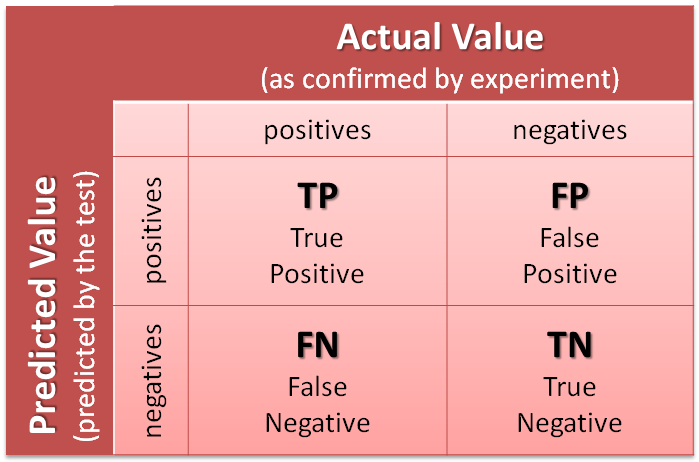
\includegraphics[width=14cm, height=7cm]{confusionmatrix.png}
\caption{Confusion Matrix representation}
\end{figure}

\subsubsection{Calcul de certains metrics de classification à partir de la matrice confusion}

La matrice de confusion en soi n'est pas une mesure de performance en tant que telle, mais presque toutes les métriques de performance sont basées sur la matrice de confusion et les nombres qui s'y trouvent. Nous allons voir comment utiliser la matrice de confusion pour calculer quelques metrics de classification.

\begin{enumerate}
\item \textbf{Accuracy:}
L'exactitude \textbf{(Accuracy en anglais)} dans les problèmes de classification est le nombre de prédictions correctes faites par le modèle sur toutes les prédictions faites.
$\textnormal{Accuracy} = \frac{TP+TN}{TP+ FP + FN + TN} $

\item  \textbf{Precision:} 
La précision permet de répondre à la question suivante : Quelle proportion d'identifications positives était effectivement correcte ?
$\textnormal{Precision} = \frac{TP}{TP+ FP} $

\item \textbf{Recall or Sensitivity:}
Le rappel permet de répondre à la question suivante : Quelle proportion de résultats positifs réels a été identifiée correctement ?
$\textnormal{Precision} = \frac{TP}{TP+ FN} $
 
 \item \textbf{F1-score:}
 Nous ne voulons pas vraiment avoir à la fois la précision et le rappel dans nos poches chaque fois que nous faisons un modèle pour résoudre un problème de classification. Donc, il est préférable que nous puissions obtenir un seul score qui représente à la fois la précision (P) et le rappel (R)
 
 $ \textnormal{F1score} = \frac{ 2 }{\frac {1}{\textnormal{precision}} +  \frac {1}{\textnormal{recall}}  } = 2 \times \frac{\textnormal{precision} \times \textnormal{recall}} { \textnormal{precision} + \textnormal{recall} } = \frac{TP} {TP + \frac{FN+FP} {2} } $
 
 \item \textbf{ROC-AUC:}
Une courbe ROC (receiver operating characteristic) est un graphique représentant les performances d'un modèle de classification pour tous les seuils de classification. Cette courbe trace le taux de vrais positifs \textbf{(True Positifs en anglais)} en fonction du taux de faux positifs \textbf{(False Positifs en anglais)}.
\end{enumerate}

\subsubsection{Classes déséquilibrées}

Nous terminerons le chapitre sur la classification en abordant un sujet très important en machine learning, surtout dans le problème de la classification qui est "\textit{Jeux de données déséquilibré}" \textbf{(Imbalanced datasets or Imbalanced Classification or Imbalanced Classes, ses appellations en anglais)}. C'est un problème très commun en machine learning, spécialement en classification. Nous abordons ce sujet parce que c'était l'une des principales difficultés de notre projet. \\

Une distribution de classe déséquilibrée est un scénario où le nombre d'observations appartenant à une classe est significativement inférieur à celui des autres classes. 
Ce problème prédomine dans les cas où la détection d'anomalies est cruciale comme le vol d'électricité, les transactions frauduleuses dans les banques, l'identification de maladies rares, etc. Dans ce cas, le modèle prédictif développé avec des algorithmes conventionnels pourrait être biaisé et inexact.\\
Cela arrive parce que les algorithmes d'apprentissage automatique sont généralement conçus pour améliorer la précision en réduisant l'erreur. Ainsi, ils ne tiennent pas compte de la répartition / proportion des classes ou de l'équilibre des classes.\\

Plusieurs techniques ont été proposées pour manipuler les classes déséquilibrées. Voyons un bref résumé de quelques-unes d'entre elles:
\paragraph{Random Under-Sampling:}
Le Random Under-Sampling vise à équilibrer la distribution des classes en éliminant de manière aléatoire les exemples de classes majoritaires. Ceci est fait jusqu'à ce que les instances de la majorité et de la classe minoritaire soient équilibrées.
\paragraph{Random Over-Sampling:}
Le Random Over-Sampling augmente le nombre d'instances dans la classe minoritaire en les reproduisant aléatoirement afin de présenter une représentation plus élevée de la classe minoritaire dans l'échantillon.
\paragraph{Cluster-Based Over Sampling:}
Dans ce cas, l'algorithme de clustering K-means est appliqué indépendamment aux instances de classe minoritaire et majoritaire. Cela permet d'identifier les clusters dans l'ensemble de données. Par la suite, chaque grappe est suréchantillonnée de sorte que tous les clusters de la même classe ont un nombre égal d'instances et toutes les classes ont la même taille.
\paragraph{Synthetic Minority Over-sampling Technique(SMOTE):}
Cette technique est suivie pour éviter le surapprentissage qui se produit lorsque des répliques exactes d'instances minoritaires sont ajoutées à l'ensemble de données principal. Un sous-ensemble de données est pris à partir de la classe minoritaire à titre d'exemple, puis de nouvelles instances similaires synthétiques sont créées. Ces instances synthétiques sont ensuite ajoutées à l'ensemble de données d'origine. Le nouvel ensemble de données est utilisé comme un échantillon pour former les modèles de classification.
\paragraph{Modified synthetic minority oversampling technique (MSMOTE):}
C'est une version modifiée de SMOTE. SMOTE ne tient pas compte de la distribution sous-jacente de la classe minoritaire et des bruits latents dans l'ensemble de données. Pour améliorer les performances de SMOTE, une méthode modifiée MSMOTE est utilisée.\\

Dans notre projet nous avons opté pour la technique de SMOTE parce qu'elle permet d'atténuer le problème de sur-adaptation \textbf{(overfitting en anglais)} causé par le sur-échantillonnage aléatoire \textbf{(random oversampling, en anglais)}
 




%\begin{table}[htp]
%\caption{Confusion Matrix}
%\begin{center}
%\begin{tabular}{|c|c|}
%
%\hline
%
%\hline
%
%\hline
%
%\hline
%
%\end{tabular}
%\end{center}
%\label{default}
%\end{table}%







\newpage

\section{Aperçu}
Pour développer notre projet, nous avons fait le cycle complet d'un data scientist. Depuis l'obtention des données jusqu'au déploiement d'un système en production. Dans ce chapitre nous allons parcourir toutes les étapes du développement de notre projet. 

\subsection{Obtention des données}
\subsection{Nettoyage des données}
\subsection{Exploration des données}
\subsection{Modélisation des données}
\subsection{Déploiement de modèle}
\subsubsection{Construction d'un API}



\newpage

\section{Évaluation}


\newpage

\section{Limitations et travaux futurs}

\newpage

\section{Travaux connexes}


\newpage

\section{Conclusion}
	
\end{document}
